% =====================================================================
%  Livrable 1 : question de recherche, collecte, description du dataset,
%  prétraitement, faisabilité. Chiffres mis à jour le 09/11/2026 avec le code
%  local (manifestes/niveau2_2026-11-09.json, niveau3_2026-11-09.json),
%  analyse/description.py et analyse/faisabilite.py.
% =====================================================================

\section{Question de recherche}

Les agences publient la liste des pénuries de médicaments en cours, jamais de prévision : patients et soignants les
découvrent une fois la rupture installée. Notre question principale :

\begin{quote}
\large\textbf{Quelles substances actives risquent de manquer en France dans les trois prochains mois, et quels facteurs
expliquent leur vulnérabilité} : criticité du médicament, niveau de demande, historique de pénuries, propagation à
partir des substituts, pénuries déjà observées chez nos voisins européens ?
\end{quote}

Nous la mesurons ainsi : une substance fera-t-elle l'objet d'\textbf{au moins un signalement de rupture à l'ANSM dans les
trois mois}, d'après les seules informations déjà publiques ? Prévoir quelles substances sont menacées permettrait
d'anticiper les tensions d'approvisionnement ; comprendre pourquoi, d'agir sur les causes. Deux mécanismes sont testés :

\begin{quote}
\large\textbf{Q1, effet cascade.} Une rupture se propage-t-elle aux substances de la même classe, qui servent de
substituts ?\par\smallskip
\large\textbf{Q2, pénuries importées.} Une pénurie déjà publiée en Italie, en Suède, en Tchéquie, en Slovaquie, en Norvège
ou en Allemagne annonce-t-elle la pénurie française ?
\end{quote}

Périmètre : la France (seul pays avec tous les médicaments commercialisés) et 885 substances à médicament
d'intérêt thérapeutique majeur (MITM, seules soumises à déclaration) délivrées en ville ; six pays européens servent de signaux.

\section{Collecte et construction du dataset}

Toutes les données viennent de sources officielles et publiques : ANSM, BDPM, Open Medic et Medic'AM pour la France ;
AIFA, BfArM, DMP, Läkemedelsverket, SÚKL et ŠÚKL pour l'Italie, l'Allemagne, la Norvège, la Suède, la Tchéquie et la
Slovaquie. Les listes ne montrent que le \emph{présent} : pour le passé, nous avons récupéré les \textbf{archives de la
Wayback Machine} (dont l'ancien site de l'ANSM, 2015-2021) ; la Suède, la Tchéquie et la Slovaquie publient des registres
historiques complets (tableau~\ref{tab:pays}).

\textbf{Une construction en trois niveaux}, comme un entrepôt de données : nous y appliquons les éléments du cours
\emph{Building a Dataset from a Warehouse} et du TP MegaStore.

\vspace{4pt}
\begin{center}
\begin{tikzpicture}[
  niveau/.style={rounded corners=6pt, fill=#1!9, draw=#1!35, line width=0.6pt, align=center, font=\small,
                 text width=5.0cm, minimum height=1.6cm, inner sep=5pt,
                 execute at begin node={\hyphenpenalty=10000\exhyphenpenalty=10000},
                 drop shadow={opacity=0.12, shadow xshift=0.6pt, shadow yshift=-0.8pt}},
  titre/.style={fill=#1, text=white, font=\footnotesize\bfseries, rounded corners=3pt, inner xsep=6pt,
                inner ysep=2.5pt, text height=1.9ex, text depth=0.5ex, anchor=south west},
  fleche/.style={-{Latex[length=5pt, width=6pt]}, line width=1.4pt, gray!45}]
\node[niveau=niveaubrut] (brut) {environ 800 fichiers sources, gardés tels quels, en lecture seule, et tracés (adresse, date, empreinte)};
\node[niveau=niveaupropre, right=0.5cm of brut] (propre) {25 tables en étoile : \textbf{grain} vérifié, médicaments
  \textbf{historisés} (jointure \emph{as-of}), \textbf{contrôles} et manifeste};
\node[niveau=niveaufinal, right=0.5cm of propre] (final) {\textbf{panel\_fr} : 58\,410 lignes (substance $\times$ mois), variables connues avant, cible après};
\node[titre=niveaubrut] at ([xshift=6pt, yshift=2pt]brut.north west) {1 \enspace BRUT};
\node[titre=niveaupropre] at ([xshift=6pt, yshift=2pt]propre.north west) {2 \enspace NETTOYÉ};
\node[titre=niveaufinal] at ([xshift=6pt, yshift=2pt]final.north west) {3 \enspace FINAL};
\draw[fleche] (brut) -- (propre);
\draw[fleche] (propre) -- (final);
\end{tikzpicture}
\end{center}
\vspace{4pt}

\section{Le dataset}

\begin{figure}[H]
\centering
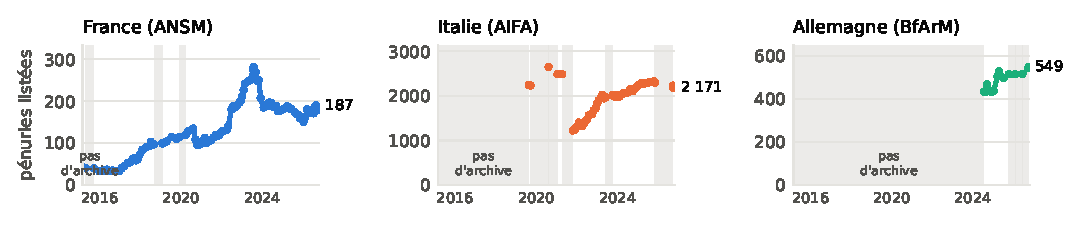
\includegraphics[width=0.78\linewidth]{figures/evolution_penuries.pdf}
\caption{Pénuries en cours par archive, pays observés par photos (zones grises : plus de 100 jours sans archive).}
\label{fig:evolution}
\end{figure}

\begin{minipage}[c]{0.47\linewidth}
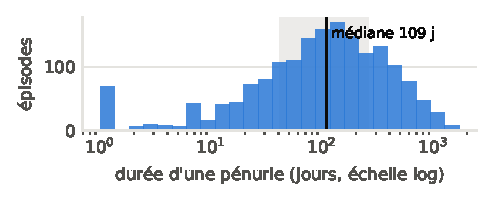
\includegraphics[width=\linewidth]{figures/durees_france.pdf}
\end{minipage}\hfill
\begin{minipage}[c]{0.51\linewidth}\small
\textbf{Durées (France, \textbf{1\,754} pénuries terminées).} Distribution asymétrique (moyenne 192\,j, médiane \textbf{109\,j},
quartiles \textbf{41 et 257\,j}, \textbf{16\,\%} au-delà d'un an) : nous retenons médiane et quartiles, pas la moyenne. Les valeurs extrêmes
sont conservées, car exceptionnelles mais exactes.
\end{minipage}

\smallskip
\textbf{39\,\%} des substances commercialisées ont connu une pénurie en France depuis 2015. Les signalements suivent la
consommation (Spearman \textbf{0,61}) et le nombre de présentations (\textbf{0,79}) : lien confondu.

\begin{table}[H]
\centering\footnotesize
\renewcommand{\arraystretch}{1.2}
\rowcolors{2}{white}{niveaubrut!6}
\begin{tabularx}{\linewidth}{>{\raggedright\arraybackslash}p{1.8cm} >{\raggedright\arraybackslash}X r r >{\raggedright\arraybackslash}p{2.6cm}}
\rowcolor{niveaubrut!16}
\entete{Pays} & \entete{Archives} & \entete{Pénuries (en cours)} & \entete{Substances · ATC} & \entete{Période} \\
France & 116 photos & 2\,764 (187) & 613 · 88,8\,\% & 02/2015--10/2026 \\
Italie & 54 photos & 13\,651 (2\,171) & 1\,136 · 91,0\,\% & 08/2019--10/2026 \\
Suède & registre ouvert & 14\,672 (880) & 1\,202 · 91,4\,\% & 02/2018--11/2026 \\
Tchéquie & déclarations & 16\,235 (1\,239) & 1\,131 · 95,3\,\% & 01/2018--11/2026 \\
Slovaquie & déclarations & 7\,651 (887) & 922 · 96,4\,\% & 04/2019--11/2026 \\
Norvège & 6 registres annuels & 6\,413 (424) & 885 · 97,2\,\% & 2019--07/2024 \\
Allemagne & 13 photos & 2\,000 (549) & 509 · 96,8\,\% & 07/2024--10/2026 \\
\filet
\end{tabularx}
\caption{Description par pays (pénuries seules, hors arrêts de commercialisation).}
\label{tab:pays}
\end{table}

\begin{table}[H]
\centering\footnotesize
\renewcommand{\arraystretch}{1.2}
\rowcolors{2}{white}{niveaubrut!6}
\begin{tabularx}{\linewidth}{>{\raggedright\arraybackslash}p{2.4cm} >{\raggedright\arraybackslash}p{4.5cm} r >{\raggedright\arraybackslash}X}
\rowcolor{niveaubrut!16}
\entete{Table} & \entete{Une ligne =} & \entete{Lignes $\times$ col.} & \entete{Variables principales} \\
Épisodes de pénurie & une pénurie d'un médicament dans un pays (7 pays) & 72\,221 $\times$ 18 &
\var{atc5} substance (clé commune) ; \var{atc4} classe de substituts ; \var{debut}, \var{fin} ;
\var{publication} date où elle devient connue ; \var{gravite}, \var{raison} \\
Signalements & un signalement d'un laboratoire, 2019--2025 & 22\,501 $\times$ 9 &
\var{date\_signalement}, \var{laboratoire}, \var{atc5} \\
Médicaments & un médicament de la BDPM & 15\,883 $\times$ 16 & \var{forme}, \var{voies},
\var{titulaires}, \var{atc5} \\
Consommation & une substance et un mois (Medic'AM, 2015--06/2026) & 161\,754 $\times$ 6 & \var{boites}, \var{montant\_rembourse} \\
Panel (niveau 3) & une substance MITM en ville par mois, 04/2020--09/2025 & 58\,410 $\times$ 25 &
\var{cible}, \var{cible\_nouvelle\_12m} ; Q1, Q2 : signaux sur 3 mois \\
\filet
\end{tabularx}
\caption{Tables principales (25 au niveau 2 + le panel) : une ligne, dimensions, variables.}
\label{tab:dataset}
\end{table}

\section{Prétraitement et choix}

\textbf{Photos et déclarations en épisodes.} Les photos successives d'un médicament forment un épisode (Italie : présence
continue, l'AIFA révisant les dates) ; en Tchéquie et en Slovaquie, une interruption déclarée ouvre l'épisode, la reprise le
ferme. Arrêts définitifs distingués ; archives tronquées écartées.

\textbf{Qualité.} Substance (ATC) retrouvée en croisant boîte, nom et substance (\textbf{9 lignes sur 10}). Aucun doublon d'épisode ni boîtes nulles. Fin vide = pénurie en cours (\textbf{7\,\%} en France, \textbf{27\,\%} en
Allemagne) ; ATC absent (\textbf{3 à 11\,\%}) = hors jointures ; \textbf{55} durées nulles gardées ; aucune imputation.
\textbf{Pas de futur} : chaque variable ne lit que ce qui était publié à la fin du mois (contrôlé par recalcul).

\section{Faisabilité et limites}

La cible vaut 1 pour \textbf{31\,\%} des lignes (\textbf{17\,929} sur 58\,410). Elle est surtout prédite par la
\textbf{répétition} : le cumul des signalements passés, seul, donne une AUC de \textbf{0,852} (0,861 avec tous les signaux). Nous retenons donc
une cible plus exigeante : une rupture sur une substance \textbf{sans signalement depuis 12 mois} (9\,\% des 27\,718 lignes
concernées). Sur cette cible (test 2025), la régression logistique passe de 0,683 à \textbf{0,702} avec les signaux européens
(Italie surtout ; gain significatif, IC 95\,\% [0,002 ; 0,037]), Q1 n'apporte rien.

\textbf{Limites.} Peu de nouvelles ruptures distinctes (587 à l'entraînement, 84 au test) ; cohorte fondée sur la liste MITM
de 2026, substances hospitalières exclues (consommation inconnue) ; taux de positifs en hausse (21\,\% en 2020, 37\,\% en 2023),
en partie par effet de déclaration ; définition de la pénurie variable selon les pays.
